% This must be in the first 5 lines to tell arXiv to use pdfLaTeX, which is strongly recommended.
\pdfoutput=1
% In particular, the hyperref package requires pdfLaTeX in order to break URLs across lines.

\documentclass[11pt]{article}

% Remove the "review" option to generate the final version.
\usepackage{acl}

% Standard package includes
\usepackage{times}
\usepackage{latexsym}
\usepackage{inconsolata}
\usepackage{amsfonts}
\usepackage{soul}
\usepackage{colortbl}
\usepackage{multirow}
\usepackage{xspace}
\usepackage{amsmath}
\usepackage{graphicx}
\usepackage{booktabs}


\newcommand{\biasbranch}{bias-only branch\xspace}
\newcommand{\originalbranch}{original branch\xspace}
\newcommand{\mc}[2]{\multicolumn{#1}{c}{#2}}
\newcommand{\swap}[3][-]{#3#1#2} 
\newcommand{\std}[1]{{\scriptsize{$\pm$#1}}}
\newcommand{\xhdr}[1]{\vspace{0em}\noindent{{\bf #1.}}}
\newcommand{\na}{~~~~~~~N/A~~~~~~~~}

\newcommand{\FT}{\textsc{FineTune}\xspace}
\newcommand{\MASK}{\textsc{DebiasMask}\xspace}
\newcommand{\KW}{\textsc{KernelWhitening}\xspace}
\newcommand{\ETE}{\textsc{E2E-PoE}\xspace}
\newcommand{\etefocal}{\textsc{E2E-Focal}\xspace}
\newcommand{\RUBI}{\textsc{RUBi}\xspace}
\newcommand{\IE}{\textsc{IEGDB}\xspace}
\newcommand{\READ}{\textsc{READ}\xspace}
\newcommand{\OursName}{\textsc{FairFlow}\xspace}
\newcommand{\OursPoe}{\OursName-\textsc{poe}\xspace}
\newcommand{\OursFocal}{\OursName-\textsc{focal}\xspace}
% \newcommand{\OursCL}{\OursName-\textsc{cl}\xspace}
\newcommand{\OursCL}{\OursName}

\newcommand{\jiali}[1]{{\color{blue}[[J: #1]]}}
\newcommand{\hadi}[1]{{\color{orange}[H: #1]}}

% For proper rendering and hyphenation of words containing Latin characters (including in bib files)
\usepackage[T1]{fontenc}
% For Vietnamese characters
% \usepackage[T5]{fontenc}
% See https://www.latex-project.org/help/documentation/encguide.pdf for other character sets

% This assumes your files are encoded as UTF8
\usepackage[utf8]{inputenc}

% This is not strictly necessary and may be commented out.
% However, it will improve the layout of the manuscript,
% and will typically save some space.
\usepackage{microtype}

% This is also not strictly necessary and may be commented out.
% However, it will improve the aesthetics of text in
% the typewriter font.
\usepackage{inconsolata}


% If the title and author information does not fit in the area allocated, uncomment the following
%
%\setlength\titlebox{<dim>}
%
% and set <dim> to something 5cm or larger.

% \title{Contrastive-based Multiview Dataset Bias Mitigation for Natural Language Processing}
\title{\OursName: Mitigating Dataset Biases through Undecided Learning\\for Natural Language Understanding} %: A Multiview Contrastive Framework for Robust Debiasing

% Author information can be set in various styles:
% For several authors from the same institution:
% \author{Author 1 \and ... \and Author n \\
%         Address line \\ ... \\ Address line}
% if the names do not fit well on one line use
%         Author 1 \\ {\bf Author 2} \\ ... \\ {\bf Author n} \\
% For authors from different institutions:
% \author{Author 1 \\ Address line \\  ... \\ Address line
%         \And  ... \And
%         Author n \\ Address line \\ ... \\ Address line}
% To start a separate ``row'' of authors use \AND, as in
% \author{Author 1 \\ Address line \\  ... \\ Address line
%         \AND
%         Author 2 \\ Address line \\ ... \\ Address line \And
%         Author 3 \\ Address line \\ ... \\ Address line}

\author{Jiali Cheng \and Hadi Amiri \\
  University of Massachusetts Lowell \\
  \texttt{\{jiali\_cheng, hadi\_amiri\}@uml.edu}
\\}

\begin{document}
\maketitle



%Recent research has discovered that fine-tuned 
\begin{abstract}
    
Language models are prone to dataset biases, known as shortcuts and spurious correlations in data, which often result in performance drop on new data. We present a new debiasing framework called ``\OursName'' that mitigates dataset biases by learning to be {\em undecided} in its predictions for data samples or representations associated with known or unknown biases. The framework introduces two key components: a suite of data and model perturbation operations that generate different biased views of input samples, and a contrastive objective that learns debiased and robust representations from the resulting biased views of samples. Experiments show that \OursName outperforms existing debiasing methods, particularly against out-of-domain and hard test samples without compromising the in-domain performance\footnote{Our code is available at \url{https://github.com/CLU-UML/FairFlow}.}.
\end{abstract}

% Existing debiasing methods mainly focus on detecting and re-weighting potentially biased samples in datasets. However, they have limited coverage of different types of biases and less regularization strength. 
% \OursName encodes less biases in its learned representations compared to strong baselines. 
% We illustrate that existing baselines are still biased and can be further debiased with our framework.
% , by modeling more sources of biases. 
%xx, xx .  % By explicitly modeling known biases, the proposed framework enhances the effectiveness of existing debiasing approaches. 
% We discuss how several existing approaches can be considered as special cases of \OursName.

\section{Introduction}

 % have been successful across a wide range of NLP tasks. %, paraphrase identification, sentiment analysis and relation extraction.  However, 
Existing computational models developed for natural language processing (NLP) tasks are vulnerable to dataset biases and spurious correlations in data, often referred to as ``shortcuts.''  % or annotation artifacts. 
These shortcuts enable models to achieve high performance on NLP datasets by exploiting surface-level correlations between features and labels. However, they also result in a significant performance drop on hard or slightly modified test data~\citep{naik-etal-2018-stress}. For example, in the area of natural language inference (NLI), models like BERT~\citep{devlin-etal-2019-bert} tend to misclassify premise-hypothesis pairs that contain ``negation'' words in their hypotheses as ``contradiction,'' which happen to be predictive features associated with the \textit{contradiction} label in certain NLI datasets~\citep{gururangan-etal-2018-annotation,poliak-etal-2018-hypothesis,modarressi-etal-2023-guide}.

% \hadi{related work, what has been done and what are the known findings. What's missing. cite all key papers.}

\begin{figure}[t]
    \centering
    \vspace{-20pt}
    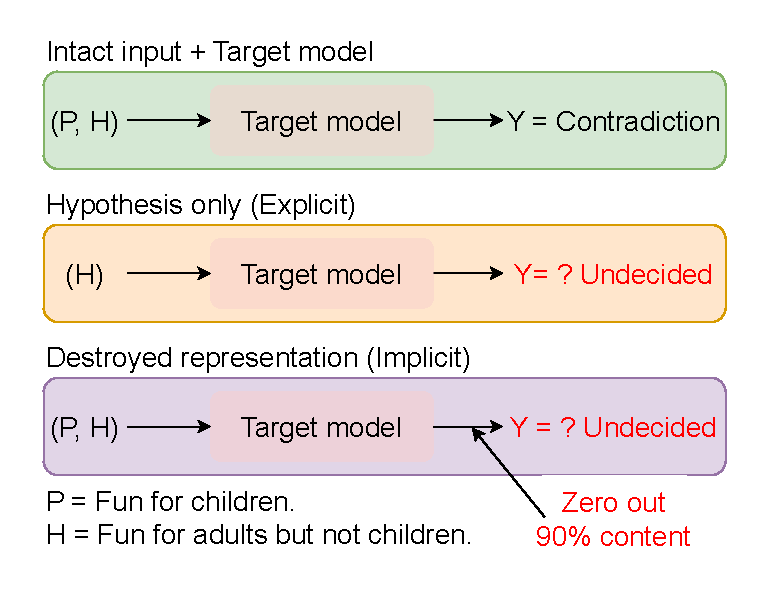
\includegraphics[width=.45\textwidth]{figure/motivating_example.pdf}
    % \vspace{-10pt}
    \caption{An example highlighting the concept of ``undecided learning'' using two types of data perturbation techniques. Given a premise-hypothesis pair in NLI, the model is expected to correctly classify their entailment relationship. However, given only the 
    % a grammatically perturbed 
    hypothesis, a robust model should be undecided, i.e., refrain from making a definite judgment 
    about the relationship between an unknown premise and %perturbed 
    the given hypothesis. Similarly, given a severely corrupted representation, a robust model should be undecided about the relation between a corrupted premise and hypothesis pair.
    Models that retain confidence in assigning labels to such inputs are likely to rely on shortcuts. \OursName takes an undecided stance against such inputs.}
    \label{fig:motivating_example}
    \vspace{-10pt}
    \label{fig:example}
\end{figure}

Existing debiasing approaches %employ external models to 
can detect known~\citep{clark-etal-2019-dont,sanh2020learning,karimi-mahabadi-etal-2020-end,modarressi-etal-2023-guide} and previously unidentified or unknown~\citep{utama-etal-2020-towards,sanh2020learning} biases in training data.
They mitigate dataset biases by 
re-weighting examples~\citep{sanh2020learning,karimi-mahabadi-etal-2020-end}, 
learning robust representations~\citep{gao-etal-2022-kernel,du-etal-2023-towards}, 
learning robust feature interaction patterns~\citep{wang-etal-2023-robust}, or 
reducing the effect of biased model components~\citep{meissner-etal-2022-debiasing}.

% Comments
% Existing
% (the original model)
% (external representations) 
% (parts)
% Any other approaches?

% \hadi{the need to investigate the missing parts. and how you do that.}s
% There are several key challenges that may compromise the effectiveness of existing approaches in mitigating dataset biases. 
Despite the significant progress made in addressing dataset biases, existing models have certain limitations:
\textbf{(a)}: they often adopt a {\em single view} to dataset biases and primarily focus on specific types of biases~\citep{clark-etal-2019-dont,karimi-mahabadi-etal-2020-end}. However, rich sources and diverse types of dataset biases can be present in the data.
\textbf{(b)}: existing approaches that are based on weak learners~\citep{utama-etal-2020-towards,sanh2020learning,ghaddar-etal-2021-end,meissner-etal-2022-debiasing} rely on a {\em single} weak learner to identify biases, which inevitably tie their performance to the capabilities of the chosen weak learner.
\textbf{(c)}: prior works often evaluate debiasing methods using BERT-based models, which may limit their generalizability to other model architectures. 

% which largely bounds these approaches by the learning capability of the weak learner.
% to insufficient regularization of model parameters against biased examples or cascade biases throughout the multi-stage training process. 
%debiasing
% Finally, existing methods are often tailored to specific NLP tasks due to the reliance on task-specific model architectures, which can restrict the transferability of the methods to different domains or problem settings. For example, Debias Mask~\citep{} does not work for embedding models, such as TransE~\citep{}. 
% We want to attend to bias when needed. 

% \hadi{2--3 key,contributions.}
We tackle the above challenges by developing \OursName--a multiview contrastive learning framework that mitigates dataset biases by being {\em undecided} in its prediction for biased views of data samples (see \textbf{Figure~\ref{fig:example}}). Specifically, the proposed method employs several data perturbation operators to generate biased views of intact data samples and integrate them into the training data and learning process. 
When presented with biased inputs, the model is trained to be undecided about the possible labels by making a uniform prediction across the label set. At the same time, the model is encouraged to be confident about intact inputs, which {\em often} serve as a reference for unbiased samples. Therefore, the approach encourages learning representations that are more attentive to the true signal of the underlying tasks rather than relying on shortcuts that are specific to certain datasets. 
In addition, the inherent randomness of the implicit perturbations in FairFlow (\S\ref{sec:imp_bias}) exposes the model to a diverse range of perturbations and prevents it from overfitting to specific types of biases present in the data.\looseness-1

The contributions of this paper are: 
\begin{itemize}
    \itemsep-1pt 
    % \itemindent-10
    \item categorization of dataset biases: we categorize prevalent data biases in NLU and model them using data perturbation operations;
    
    \item bias mitigation as an ``undecided learning'' problem: we formulate the bias mitigation problem as an ``undecided learning'' problem, which encourages reliance on genuine and task-related signals for effective debiasing;  
    % the approach can be applied to existing debiasing strategies in prior research. 
    %Specifically, in the presence of biased inputs, our approach ensures that the model's predictions are uniform across the label set, while it remains confident in predicting the labels of intact--mainly unbiased--data samples.
    \item robust performance on challengng samples: our approach shows robust results on {\em harder} test data while maintaining strong in-domain performance across several NLU tasks.\looseness-1
    % \item Our framework employs the Attention mechanism and can learn when to attend to bias and when not to. It also serves as an interpretability tool to recognize and classify spurious data.
    % \item Our framework is flexible to work with many debiasing strategies, including Product of Experts (PoE), Focal Loss (FL), etc.
    % \item We conduct extensive experiments on various types of NLP tasks, uncovering the disadvantages existing debias methods.
\end{itemize}

The experimental results show that \OursName obtains substantial improvement over competing models. Specifically, it achieves an average performance gain of 10.2 points on stress test datasets across several NLU tasks while maintaining performance on the original test sets. In addition, models trained using our framework show strong transferability, resulting in an average gain of 3.7 points in transfer testing experiments across different datasets and domains. 
Furthermore, 
% Our findings shed light on the biases present in existing debiasing methods, which still leave room for enhancement. Specifically, 
we show that existing methods can be further improved by incorporating the proposed perturbation operators within their original objectives, resulting in a substantial average improvement of 5.8 points on stress test sets across datasets. 
% with Product of Experts~\citep{10.1162/089976602760128018}. 
% In addition, we illustrate that existing debiasing methods still rely on shortcuts.



\begin{figure*}[t]
    \centering
    \vspace{-20pt}
    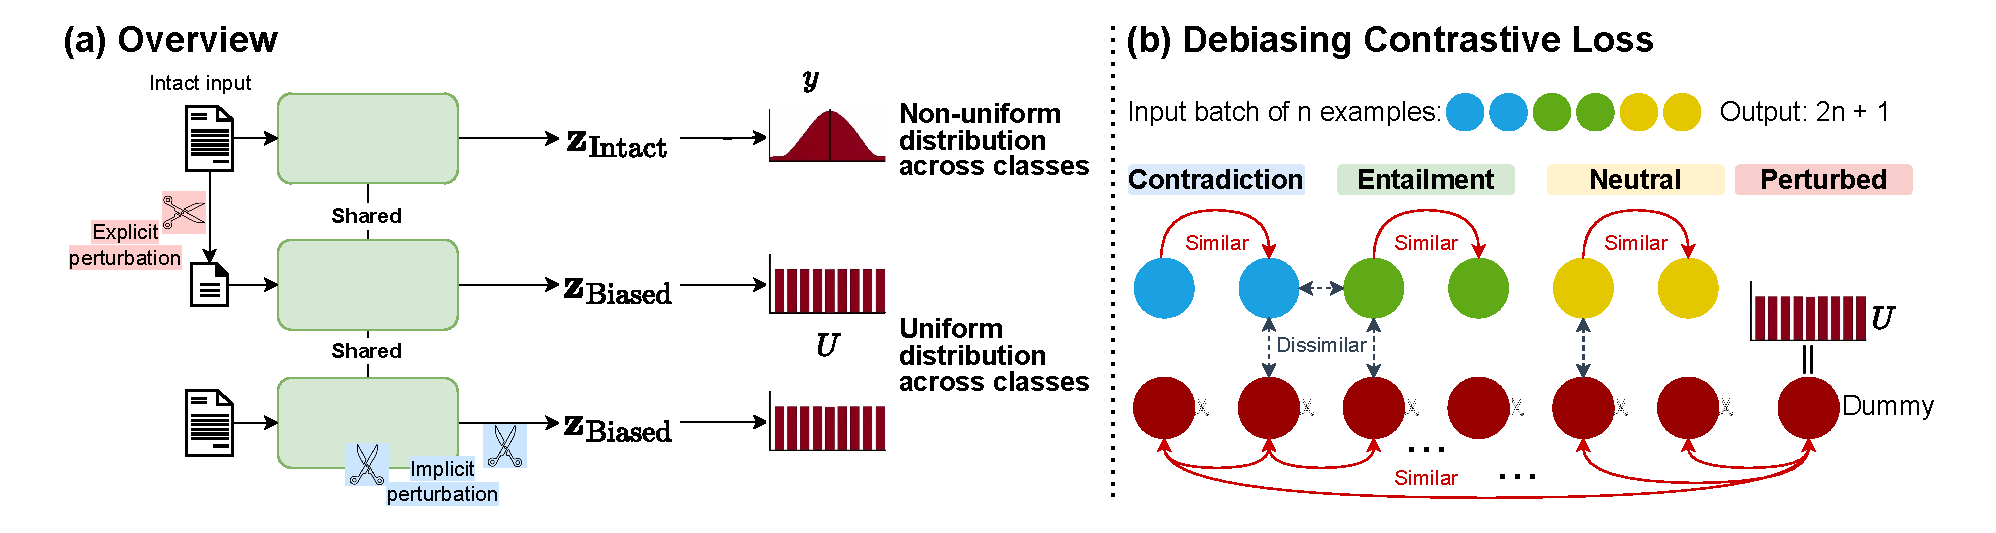
\includegraphics[width=.9\textwidth]{figure/fairflow.pdf}
    % \vspace{-20pt}
    \caption{Architecture of the proposed model. (a) Explicit and implicit perturbations are applied to inputs to obtain biased prediction $z_{\mathrm{Biased}}$. (b) Biased predictions are drawn closer to uniform distribution, while predictions for intact input are pushed away from uniform distribution through contrastive learning.}
    \label{fig:model}
    % \vspace{-10pt}
\end{figure*}

\section{Method}
\subsection{Problem Formulation}
We consider a dataset $\mathcal{D} = \{(x_i, y_i)|_{i=1}^n\}$, where $x_i$ is the $i$-th input consisting of several constituents $x_i = (x_i^1, x_i^2, \dots, x_i^p), |x_i| = p > 1$, and $y_i$ is the corresponding output for $x_i$. For example, in case of NLI, $p=2$ represents premise and hypothesis in each input and $y_i$ reflects the entailment or no-entailment relationship between the input pair. Our goal is to develop a model that is robust against different types of dataset biases in $\mathcal{D}$. 
We note that the model can be applied to a more general setting where input $x_i$ does not explicitly consist of several constituents, see \S\ref{sec:explicit_bias}.

% \subsection{A Motivating Example}
% As Figure~\ref{fig:motivating_example} shows, when given an intact premise-hypothesis pair, we want to train an NLI model to be determined about the label, since the input contains full information about the relationship between the input pair. However, if the input only contains the premise, the model should not be able to infer any information about the relationship between the premise and the hypothesis, because the hypothesis is missing. Even though the premise itself is still a valid sentence, it does not allude any signal about its relationship with another absent sentence. If a model is still confident about a label given partial input, it is very like that it relies on shortcuts to make predictions. Therefore, given such \textit{significantly corrupted instances or representations}, a robust model should remain \textit{undecided about the label}, encouraging itself to focus on causal signals rather than spurious shortcuts.


\subsection{Overview}
We categorize dataset biases as \textit{explicit} and \textit{implicit} biases. Explicit biases are readily discernible and understandable by humans, such as high degree of lexical overlap between the premise and hypothesis in case of NLI. On the other hand, implicit biases are often subtle, indiscernible to humans, and more challenging  
%linguistic (lexical or syntactic) 
% characteristics are unknown
to detect. For example, any word in input has the potential to act a shortcut, resulting in spurious correlations. 
We introduce different types of explicit and implicit biases that are {\em task-independent} and generally applicable to bias mitigation across NLP datasets (\S\ref{sec:biasmodeling}). 
%
Given such categorization, we propose a debiasing framework that mitigates dataset biases by learning genuine task-related representations that are attentive to the true signal of the tasks rather than biases and shortcut solutions in datasets. 
The key novelty of our approach is in imposing a downstream model to adopt an ``undecided'' (``uncertain'') stance in its predictions when presented with biased views of inputs. The framework achieves this goal by assigning a uniform probability across the labels, see \textbf{Figure~\ref{fig:model}}. 
Specifically, the model regularizes the loss of the target task with a contrastive loss which draws biased predictions closer to a uniform distribution while pushing other predictions away from uniform distribution (\S\ref{sec:contrastive}).  
%



% \paragraph{Bias Categorization}

% \hadi{explain/justify why each type should be considered for debiasing and how it contributes to debiasing.}

% . Some are not human perceivable. We term these biases as implicit biases. In addition to the above explicit biases, there exist other types of biases that are not as explicit as lexical or subpart bias. Other types of biases may be hard to categorize. 

% \subsubsection{Explicit Biases}
% \paragraph{Sub-input bias (explicit)} 



\subsection{Bias Modeling}\label{sec:biasmodeling}
We present a series of data perturbation operations to generate biased views by corrupting intact inputs. These perturbations can be explicit or implicit. In explicit perturbation, we directly corrupt the input data, while in implicit perturbation, we corrupt the representations of the input data. These perturbation techniques impose controlled variations on the data, which enable us to conduct a thorough analysis of their effects on bias mitigation.



% We first propose a set of data perturbations that explicitly perturb the input data. Then we model the biases in these explicitly perturbed data to force our model to make uniform predictions. We consider several types of known biases: 

\subsubsection{Explicit Biases} \label{sec:explicit_bias}
% We introduce Sub-input and Ungrammatical explicit perturbations. 

% \hadi{re lexical overlap and negation perturbations: these are tasks specific.. also, our stress sets includes these.. so our eval won't be fair as we are directly optimizing on biases that we know exist in test sets. }

% we propose a set of data perturbation operations that explicitly perturb the input data. Then we model the biases in these explicitly perturbed data and force our model to make uniform predictions.
\paragraph{Ungrammatical Perturbation} Recently, \citet{sinha-etal-2021-unnatural} showed that traditional and recent neural language models can be largely invariant to random word order permutation in their inputs. 
An ungrammatical input is often not understandable by humans and can potentially lead to explicit biases when models confidently predict outcomes for such inputs. For example, a model making a confident prediction about the contradiction class for the following perturbed premise-hypothesis pair from Figure~\ref{fig:example} may attribute its confidence to the negation term in the hypothesis: (``{\tt children fun for}'', ``{\tt children fun adults but for not}''). 
% premise: (``{\tt children fun adults but for not}'', ``{\tt children only for fun}''). 
To obtain an input with grammatical biases, we design the perturbation operation $\mathcal{P}_{Gra}$ that 
% randomly shuffles 
corrupts the word order in each input $x_i$. We encode the shuffled input using the shared encoder $f$ and transform it with a branch-specific MLP as follows:
\begin{equation}
    z_{Gra} = \texttt{MLP}_{Gra} \Big( f\big(\mathcal{P}_{Gra}(x_i) \big) \Big).
\end{equation}


\paragraph{Sub-input Perturbation} 
In NLP tasks that involve multi-part inputs (such as NLI), it is crucial to use the information from all parts of the input for prediction, i.e., all constituents should collectively contribute to accurate prediction. More importantly, an incomplete input should not lead to a confident prediction, as important information may be removed. 
Therefore, an explicit bias arises when the model makes confident predictions based on incomplete input, such as predicting the \textit{entailment} relation when only the hypothesis is provided as input in case of NLI. Sub-input biases can arise from any part of the input, denoted as $\{x_i^j\}_{j=1}^p$, or from various text spans within different sub-parts.
To realize sub-input biases, we define the $\mathcal{P}_{Sub}$ operator that takes one of the constituents of $x_i$, which is hen encoded with a shared encoder $f$ and further transferred with a constituent-specific $\texttt{MLP}_{Sub}$ as follows:
\begin{equation}
\label{eq:sub_aug}
    z_{Sub} = \texttt{MLP}_{Sub}\Big( f\big (\mathcal{P}_{Sub}(x_i)\big) \Big).
\end{equation}

\noindent We note that this operator is applicable to a more general setting where input $x_i$ does not explicitly consist of several constituents, e.g., in general text classification problems. In such cases, each $x_i$ can be divided into $p>1$ text segments. However, we acknowledge that there are tasks in which one sub-input, i.e. ${x_i^j}$ for a specific $j$, is enough to make a correct prediction for the complete input ${x_i}$, and therefore remaining undecided may seem counter-intuitive. Nevertheless, by training the model to be undecided when presented with incomplete information, we minimize the risk of biased predictions based solely on partial information, which can, in turn, make the model more robust against potential biases associated with incomplete data. 


% \paragraph{Lexical Overlap Perturbation} 
% \paragraph{Irrelevant Text Perturbation} 
% Deep learning models are vulnerable to wording of their inputs~\citep{gururangan-etal-2018-annotation}. In fact, they may focus on specific keywords and ignore the semantic and syntax analysis that is often required to effectively process the text. To obtain an input with irrelevant text biases, we design the perturbation operation $\mathcal{P}_{Irr}$  that appends irrelevant text to all the constituents of $x^i$. We encode the perturbed input using the shared encoder $f$ and transform it with a branch-specific MLP as follows:
% \begin{equation}
%     z_{Irr} = \texttt{MLP}_{Irr} \Big( f\big(\mathcal{P}_{Irr}(x_i)\big) \Big).
% \end{equation}

% \paragraph{Negation perturbation} Specific input words can have superficial correlations with labels, such as negation words in hypothesis in case of NLI. Models are prone to focus only on such superficial correlations, ignoring information from other parts. For example, BERT tends to classify examples as \textit{contradictory} because of the negation words in the hypothesis, neglecting the entailing relation between the premise and the hypothesis~\citep{karimi-mahabadi-etal-2020-end}. %Unlike previous works~\citep{}, 
% To obtain an input with negation bias, we design an perturbation operation $\mathcal{P}_{Neg}(\cdot)$ that adds negation words to the input $x^i$ as an perturbation. We encode the perturbed input using the shared encoder $f$ and transform it with a branch-specific MLP following 
% \begin{equation}
%     z_{Neg} = \texttt{MLP}_{Neg} \Big(f\big(\mathcal{P}_{Neg}(x^i)\big)\Big).
% \end{equation}


\subsubsection{Implicit Biases}
\label{sec:imp_bias}
The idea of implicit perturbations is to obtain biased representations of intact data, without explicitly perturbing the input. We introduce model- and representation-based implicit perturbation.

\paragraph{Model-based Perturbation} This approach largely perturbs a given model by converting it into a much weaker model, using mechanisms such as sparsification and layer dropping~\citep{NEURIPS2021_6e8404c3}. A weaker model is believed to capture more biases than a stronger model~\citep{ghaddar-etal-2021-end,sanh2020learning,utama-etal-2020-towards}. While existing methods require training a weak learner in advance~\citep{utama-etal-2020-towards,sanh2020learning,meissner-etal-2022-debiasing}, our method obtains biased predictions through the same deep neural model ($f$) and can be trained \emph{end-to-end}. Formally, we design a model-based perturbation operator $\mathcal{P}_{Mod}$ that uses only the first $k$ layers of the shared encoder $f$, which results in a substantially weakened model with reduced representation power. This branch encodes the intact input using the perturbed model and transform it with a branch-specific MLP as follows:
\begin{equation}
    z_{Mod} = \texttt{MLP}_{Mod} \Big( \mathcal{P}_{Mod}(f)(x_i) \Big).
\end{equation}



\paragraph{Representation-based Perturbation} This perturbation encodes the intact input with the original encoder $f$ but significantly corrupts the generated representations. Given this severely damaged and much less meaningful representation, the model should not be able to predict the correct label. We design a representation-based perturbation operator $\mathcal{P}_{Rep}$ that corrupts the intact representation, $f(x_i)$, and creates a severely perturbed representation. We then transform the perturbed representation with a branch-specific MLP as follows:
\begin{equation}
\label{eq:rep_aug}
    z_{Rep} = \texttt{MLP}_{Rep} \Big( \mathcal{P}_{Rep} \big( f(x_i) \big) \Big).
\end{equation}


% either modeling the existing biases or creating additional biases. 



% \paragraph{Perturbation}
\textbf{Table~\ref{tab:aug_list}} summarizes the above perturbation operators and provides details of their implementations. 
% DropPremise, which drops the premise part of the input; 2) DropHypothesis, which drops the hypothesis part of the input; 3) HalfHalf, which randomly takes 50\% of the tokens from each sentence; 4) Shuffle, which randomly shuffles the premise and the hypothesis; 5) DropLayer, which drops all layers after the 2nd layer; and 6) DestroyRep, which zeros out 90\% of the elements in the intact representation.




\subsection{Supervised Contrastive Debiasing}\label{sec:contrastive}
Given the explicit and implicit biased views of data samples, we expect a robust debiasing model to maintain an ``undecided'' stance across labels for biased inputs while providing confident predictions for intact inputs $x_i, \forall i$. Based on this intuition, the outputs of the bias branches should approximate a {\em uniform distribution} ($U$) across classes, while the output of the original branch should align with its corresponding gold distribution, i.e., the label $y_i$. 
% Through back-propagation, we can achieve the goal of debiasing the representations of the backbone model. 
To achieve this goal, we adapt the supervised contrastive loss~\citep{khosla2020supervised}, which operates by first grouping samples based on their respective labels, and then encouraging predictions (logits) of pairs within the same group to become closer while pushing logits of pairs across different groups further apart, i.e. forming positive pairs within the same group while creating negative pairs using all other pairs: % (see footnote 2).
% i.e. forming positive pairs within the same group while creating negative pairs across different groups.

\begin{table}\small
\centering
\setlength{\tabcolsep}{3pt}
\renewcommand{\arraystretch}{1} 
\begin{tabular}{c|c|l}
\toprule
\textbf{Operator}               & \textbf{Type}     & \textbf{Implementation} \\
\midrule
$\mathcal{P}_{Gra}$ & Explicit & Shuffle tokens in $x_i$ randomly \\
$\mathcal{P}_{Sub}$  & Explicit & Drop $1/p$ of tokens from $x_i^j$ randomly \\
$\mathcal{P}_{Sub}$  & Explicit & Drop $x_i^j, j=1\dots p$ \\
% $\mathcal{P}_{Irr}$  & Explicit & Add same irrelevant text to all $x_i^j$ \\
% $\mathcal{P}_{Neg}$  & Explicit & Add negation words to all $x^i_p$ \\
\midrule
$\mathcal{P}_{Mod}$  & Implicit & Use only first $k$ of layers of $f$\\
$\mathcal{P}_{Rep}$  & Implicit & Zero out $m\%$ of values in $f(x_i)$ \\
\bottomrule
  \end{tabular}
  \caption{Implementations of proposed perturbations}
  \label{tab:aug_list}
  \vspace{-10pt}
\end{table}


We adapt this loss function for bias mitigation as follows (described for a single perturbation for simplicity):
given a batch of $n$ non-perturbed examples, we perturb them using a perturbation technique described in Table~\ref{tab:aug_list}. The perturbed examples form a single group as they all have the same label (a uniform distribution across all classes), and the non-perturbed examples with the same label form separate groups.\footnote{For example, four groups in case of NLI: perturbed examples, non-perturbed examples labeled as `entailment', non-perturbed examples labeled as `contradiction', and non-perturbed examples labeled as `neutral'.} 
As illustrated in \textbf{Figure~\ref{fig:model}}, we encourage the model to be undecided about the label of perturbed inputs by adding a dummy example that has a ``fixed'' uniform distribution across all labels to the group of perturbed examples, resulting in a batch of $2n+1$ examples ($\mathcal{I}$). We compute the contrastive loss as follows:
\begin{multline}
\label{eq:supcontras}
    \mathcal{L}_{\mathrm{Debias}} = \\ 
    \sum_{i \in \mathcal{I}} \frac{-1}{|\mathcal{G}(i)|} \sum_{j \in \mathcal{G}(i)} \mathrm{log} \frac{\mathrm{exp} (z_i \cdot z_j / \tau)}{\sum_{k \in \mathcal{A}(i)} \mathrm{exp} (z_i \cdot z_k / \tau)},
\end{multline}
where $\mathcal{G}(i)$ is the set of examples that are in the same group as $i$ (having the same label as $i$); 
$\mathcal{A}(i) = \mathcal{I}\backslash\{i\}$ is the set of all examples except $i$; 
$z$ indicates the logit of an example, which for perturbed examples is obtained from one of the Equations (\ref{eq:sub_aug})--(\ref{eq:rep_aug}); and 
$\tau$ denotes the temperature parameter.\footnote{We note that the summation over all samples except $i$ in the denominator of (\ref{eq:supcontras}) is motivated by noise contrastive estimation and N-pair losses~\citep{khosla2020supervised,pmlr-v9-gutmann10a,NIPS2016_6b180037}, in which the ability to discriminate between signal and noise (negative class) is improved by adding more examples of negative class.} The dummy example in the perturbed group has a fixed uniform distribution across all labels as its $z$. This formulation encourages the model to be undecided about the label of perturbed inputs, while being confident about the labels of intact inputs, allowing it to effectively distinguish between different groups of examples. 

% Given the logit of each example non-perturbed example $z_i$ from Equations \ref{eq:sub_aug}--\ref{eq:rep_aug}, ee enforce $z_{2N+1}$ to be a ``fixed'' uniform distribution across all labels, which can be thought of as adding a dummy example of uniform distribution to the group of perturbed examples. This dummy example is used for creating positive pairs for examples within the perturbed group. This adjustment enables the model to learn representations that can effectively distinguish between perturbed and non-perturbed examples. Given an index $i$, $G(i)$ denotes the indices in $I$ from the same group of $i$. The contrastive debiasing loss is defined as % If the $i$-th example is non-perturbed, $P(i)$ denotes the indices of the examples whose labels are the same as $i$'s. If the $i$-th example is perturbed, $P(i)$ denotes the indices of uniform distribution. We enforce the logits $z_p$ in the numerator of Eq.~\ref{eq:supcontras} 



% $A(i) = I\backslash\{i\}$ and $\tau$ denotes the temperature parameter. This formulation encourages the model to be undecided about the label of partial or significantly perturbed inputs, while being confident about the labels of intact inputs.



% a two-step process: 1) sample augmentation and 2) grouping based on class labels. To adapt it for bias mitigation, we follow the same process but adopt different augmentation and grouping methods. Specifically, given a batch of examples, we first perturb the examples with our proposed perturbations in Table~\ref{tab:aug_list}. Next, perturbed examples form a single group as they all have the same label (a uniform distribution across all labels), and non-perturbed examples with the same label form separate groups. For instance, in the context of the NLI task, this adaptation results in four distinct groups: perturbed examples, non-perturbed examples labeled as 'entailment', non-perturbed examples labeled as 'contradiction', and non-perturbed examples labeled as 'neutral'. Examples from the same group are encouraged to be similar, while examples across groups are encouraged to be dissimilar.

% Formally, we describe our proposed loss function with a single perturbation, which can be extended to multiple perturbations. Given a batch of $N$ examples, we randomly sample $p \in \mathcal{P}$ to transform the batch into a multiviewed batch, where $i \in I \buildrel\Delta\over = \{1, 2, ..., 2N+1 \}$ denotes the index of examples. We first obtain their representations $z_i \forall i \in I$, depending on what perturbation is applied to the example following Equations \ref{eq:sub_aug}--\ref{eq:rep_aug}, with $z_i = f(x_i)$ as the non-perturbation representation. We enforce $z_{2N+1}$ to be a ``fixed'' uniform distribution across all labels, which can be thought of as adding a dummy example of uniform distribution to the group of perturbed examples. This dummy example is used for creating positive pairs for examples within the perturbed group. This adjustment enables the model to learn representations that can effectively distinguish between perturbed and non-perturbed examples. Given an index $i$, $P(i)$ denotes the indices in $I$ from the same group of $i$. The contrastive debiasing loss is defined as % If the $i$-th example is non-perturbed, $P(i)$ denotes the indices of the examples whose labels are the same as $i$'s. If the $i$-th example is perturbed, $P(i)$ denotes the indices of uniform distribution. We enforce the logits $z_p$ in the numerator of Eq.~\ref{eq:supcontras} 
% \begin{multline}
% \label{eq:supcontras}
%     \mathcal{L}_{\mathrm{Debias}} = \\ 
%     \sum_{i \in I} \frac{-1}{|P(i)|} \sum_{p \in P(i)} \mathrm{log} \frac{\mathrm{exp} (z_i \cdot z_p / \tau)}{\sum_{a \in A(i)} \mathrm{exp} (z_i \cdot z_a / \tau)},
% \end{multline} where $A(i) = I\backslash\{i\}$ and $\tau$ denotes the temperature parameter. This formulation encourages the model to be undecided about the label of partial or significantly perturbed inputs, while being confident about the labels of intact inputs.


% $\mathcal{P}(i) \buildrel\Delta\over =  \{x^i_j\}_{j=1}^P$
% \begin{equation}
%     l = - log \frac{sim(i, j)}{\sum }
% \end{equation}
% \begin{equation}
%     \mathcal{L}_{Debias} = \mathcal{L}_{Intact} + \mathcal{L}_{Bias},
% \end{equation}
% \begin{equation} 
% \label{eq:intact}
%     \mathcal{L}_{Intact} = \mathbb{KL}(z_{Intact}||y) - \mathbb{KL}(z_{Intact}||U),
% \end{equation}
% \begin{equation}
% \label{eq:bias}
%     \mathcal{L}_{Bias} = \mathbb{KL}(z_{Bias}||U) - \mathbb{KL}(z_{Bias}||y),
% \end{equation}

% where $\mathbb{KL}(q||p)$ denotes the KL-Divergence and $U$ denotes the uniform distribution over the labels. 
% Equation \ref{eq:intact} encourages the model to be confident about the labels of intact inputs, while Equation \ref{eq:bias} encourages our model to be undecided about the labels of biased inputs.
%
Finally the model learns the debiasing task in an \emph{end-to-end} manner by minimizing the standard cross-entropy loss with predictions of intact input $z_{\mathrm{Intact}}=f(x_i)$ and the debiasing loss, weighted by a balancing hyperparameter $\lambda$ as follows:
\begin{equation}
    \theta^{*} = \arg\min_{\theta} \mathcal{L}_{\mathrm{CE}}(z_{\mathrm{Intact}}, y_i) + \lambda \mathcal{L}_{\mathrm{Debias}}.
\end{equation}




% \begin{table}\small
% \centering
% \setlength{\tabcolsep}{3.9pt}
% \renewcommand{\arraystretch}{0.9} 
% \begin{tabular}{c|c|l}
% \toprule
% Method               & Type     & Implementation \\
% \midrule
% $\mathcal{P}_{Sub}$  & Explicit & Drop $x_i^p$ \\
% $\mathcal{P}_{Sub}$  & Explicit & Drop $1/p$ of tokens from each $x^i_p$ randomly \\
% $\mathcal{P}_{Gra}$ & Explicit & Shuffle tokens in $x^i$ randomly \\
% $\mathcal{P}_{Irr}$  & Explicit & Add same irrelevant text to all $x^i_p$ \\
% % $\mathcal{P}_{Neg}$  & Explicit & Add negation words to all $x^i_p$ \\
% \midrule
% $\mathcal{P}_{Mod}$  & Implicit & Use only first 20\% of layers of $f$\\
% $\mathcal{P}_{Rep}$  & Implicit & Zero out 90\% of $f(x^i)$ \\
% \bottomrule
%   \end{tabular}
%   \caption{Implementations of proposed perturbations}
%   \label{tab:aug_list}
%   \vspace{-10pt}
% \end{table}
% Sup contras loss
% We adopt the Supervised Contrastive Learning loss~\citep{khosla2020supervised} shown in (\ref{eq:supcontras}) to achieve our contrastive learning objective:
% \begin{multline}
% \label{eq:supcontras}
%     \mathcal{L}^{sup}(z_i) = \sum_{i \in I} \mathcal{L}^{sup}_{out, i} = \\ 
%     \sum_{i \in I} \frac{-1}{|P(i)|} \sum_{p \in P(i)} \mathrm{log} \frac{\mathrm{exp} (z_i \cdot z_p / \tau)}{\sum_{a \in A(i)} \mathrm{exp} (z_i \cdot z_a / \tau)},
% \end{multline} where $A(i) \buildrel\Delta\over =  \{x^i_j\}_{j=1}^P$ denotes a multiviewed batch of the $i$-th example, $P(i)$ denotes the indices of examples in $A(i)$ whose label is the same as $i$'s, $z_i$ denotes the representation of the $i$-th example, and $\tau$ denotes the temperature parameter that is used for smoothness and hard negatives purposes~\citep{khosla2020supervised}. %...

% Given an input example $(x, y)$ with $P$ constituents in $x$, we first obtain the outputs from all the branches as described in \S\ref{sec:bias_branch}. We then apply the contrastive objective to learn debiased representations. For the output of the original branch $z_O$, we consider the uniform distribution $U$ as the negative example and the biased distribution $y$ as the positive example. For the output of any bias branch $z_B$, we consider $U$ as the positive example and $y$ as the negative example. 

% Finally, we combine the original Cross-Entropy Loss and the contrastive loss, weighted by a balancing factor $\lambda$. The final loss is defined as 
% \begin{multline}
%     \mathcal{L} = \mathcal{L}_{\mathrm{CE}}(z_O, y) + \lambda (\mathcal{L}^{sup}(z_O) + \\ \mathcal{L}^{sup}(z_L) + \mathcal{L}^{sup}(z_W) + \sum_{p} \mathcal{L}^{sup}(z_p)).
% \end{multline}


\paragraph{Compatibility and Difference with Other Debiasing Objectives and Training Methods} Our framework is designed to be %provide flexibility and adaptability 
compatible with debiasing objectives in existing literature. Notably, it can incorporate objectives such as the product of experts (PoE)~\citep{karimi-mahabadi-etal-2020-end,clark-etal-2019-dont}, debiased focal loss~\citep{karimi-mahabadi-etal-2020-end}, and other possible objectives, see Appendix~\ref{sec:debias_obj} for more details. In experiments, we show that our framework can further improve these well-performing baseline models. One major difference with existing debiasing objectives is that prior works use a biased model to measure how much biases present in input, while \OursCL encourages robust models to be undecided given known biased inputs, obtained by the proposed perturbations.
Moreover, we do not impose any restriction on the parametrization of the underlying model $f$, making our framework flexible to work with a wide range of training methods and network architectures (Table~\ref{tab:roberta}-\ref{tab:gpt2} in Appendix).


\section{Experiments}

% \subsection{Setup}
\paragraph{Setup}
We employ BERT~\citep{devlin-etal-2019-bert} as the commonly-used base model in previous works. In addition, we extend our evaluation to RoBERTa~\citep{liu2019roberta} and GPT-2~\citep{radford2019language} for a more comprehensive analysis.

\paragraph{Datasets} We evaluate our debiasing framework on three NLP datasets including 
MNLI~\citep{williams-etal-2018-broad}, 
paraphrase identification using Quora question pairs (QQP)~\citep{sharma2019natural}, and
relation extraction using gene-phenotype relation (PGR)~\citep{sousa-etal-2019-silver}. 
% We use their corresponding \textbf{In-Domain Test Sets} for evaluation.
These datasets are used for {\em in-domain} (ID) evaluation.

\paragraph{Stress Test Sets} We assess the robustness of models against spurious correlations using ``stress test sets,'' specifically designed with hard examples to challenge models. 
% We test if models are robust to spurious correlations with \textit{stress test sets} which contain hard examples created to fool models. 
We use the stress test set for MNLI from~\citep{naik-etal-2018-stress}, and
use the same approach to generate the stress test set for QQP.
% following the same label preserving rules from~\citep{naik-etal-2018-stress}. 
For PGR, the label-preserving rules from previous tasks do not apply due to the nature of this dataset.
% the above rules are not be applicable since it doesn't align with the nature of the task. However, 
However, given the long-tail distribution of entity appearances, we create a stress test set for PGR by selecting test examples in which both entities appear less than five times in the training set.

\paragraph{OOD Test Sets} We assess the performance of models on existing out-of-distribution (OOD) test sets, which serve as another challenge benchmark. For MNLI, we use HANS~\citep{mccoy-etal-2019-right}, which is designed to test models' capabilities against lexical and syntactic heuristics in data. For QQP, we employ the PAWS dataset~\citep{zhang-etal-2019-paws}, which focuses on paraphrase identification in cases of high lexical and surface-level similarity between question pairs.

\paragraph{Transfer Test Sets} We evaluate the performance of models in maintaining strong transferability across datasets. We use SNLI~\citep{bowman-etal-2015-large} and MRPC~\citep{dolan-brockett-2005-automatically} as the transfer set for MNLI and QQP, respectively. 
% \paragraph{Probing set}
% Previous work~\citep{mendelson-belinkov-2021-debiasing} discovered that debiased models can be still biased. We use the probing set to probe if there still exists dataset bias in our model.

\begin{table*}
\tiny
\centering
% \setlength{\tabcolsep}{3.9pt}
% \renewcommand{\arraystretch}{0.9} 
\begin{tabular}{l|cccc|cccc|cc|cccc}
\toprule
\multirow{2}{2em}{\textbf{Model}} & \multicolumn{4}{c|}{\textbf{MNLI} (Acc.)} & \multicolumn{4}{c|}{\textbf{QQP} (F1)} & \multicolumn{2}{c|}{\textbf{PGR} (F1)} & \multicolumn{4}{c}{\textbf{Avg.}}\\
               & ID   & Stress & OOD & Transfer & ID & Stress & OOD & Transfer & ID & Stress & ID & Stress & OOD & Transfer \\ 
    \toprule
    \textbf{\FT}        & 84.3 & 61.7 & 59.7 & 78.7 & 88.6 & 63.3 & 47.7 & 65.1 & 64.3 & 55.2 & 79.1 & 60.1 & 53.7 & 71.9 \\ 
    \midrule
    \textbf{\MASK}      & 83.5 & 59.7 & 59.7 & 78.3 & 88.1 & 64.6 & 50.3 & 68.5 & 64.1 & 51.7 & 78.6 & 58.7 & 55.0 & 73.4 \\ 
    \textbf{\KW}        & 84.0 & 60.9 & 60.2 & 78.4 & 88.8 & 65.1 & 51.2 & 69.6 & 64.3 & 51.8 & 79.0 & 59.3 & 55.7 & 74.0 \\ 
    \textbf{\ETE}       & 83.4 & 61.3 & 62.3 & 77.5 & 88.5 & 64.5 & 51.4 & 70.5 & 63.0 & 53.6 & 78.3 & 59.8 & 56.8 & 74.0 \\
    \textbf{LSWC}       & 80.7 & 59.4 & 59.3 & 77.7 & 87.1 & 65.8 & 49.6 & 70.0 & 63.3 & 52.8 & 77.0 & 59.3 & 54.5 & 73.8 \\ 
    \textbf{\IE}        & 84.1 & 61.8 & 62.7 & 78.1 & 87.6 & 63.5 & 53.0 & 68.3 & 64.2 & 54.9 & 78.6 & 60.1 & 57.9 & 73.2 \\
    \textbf{\READ}      & 80.8 & 61.5 & 63.4 & 75.1 & 87.0 & 66.7 & 53.6 & 68.2 & 63.0 & 54.4 & 76.9 & 60.9 & 58.5 & 71.7 \\ 
    \midrule
    \textbf{\OursPoe}   & 84.6 & 64.3 & 64.3 & 79.5 & 88.8 & 71.0 & 53.9 & 70.4 & 64.9 & 55.9 & 79.4 & 63.7 & 59.1 & \underline{75.0} \\ 
    \textbf{\OursFocal} & \underline{84.9} & \underline{64.8} & \underline{64.3} & \underline{79.3} & \underline{89.5} & \underline{71.3} & \underline{54.9} & \underline{70.7} & \underline{65.4} & \underline{56.5} & \underline{79.9} & \underline{64.2} & \underline{59.6} & \underline{75.0} \\
    \textbf{\OursCL}    & \textbf{85.1} & \textbf{65.4} & \textbf{64.9} & \textbf{79.6} & \textbf{90.4} & \textbf{72.0} & \textbf{56.0} & \textbf{72.4} & \textbf{65.9} & \textbf{56.6} & \textbf{80.5} & \textbf{64.7} & \textbf{60.5} & \textbf{76.0} \\ 
    \bottomrule
  \end{tabular}
  \caption{Experimental results on three datasets averaged across three architectures. Results for each architecture are shown in Table~\ref{tab:bert}-\ref{tab:gpt2} in Appendix. The best performance is in \textbf{bold} and the second best is \underline{underlined}.}
  \label{tab:main}
\end{table*}


\begin{table*}
\small
\centering
\begin{tabular}{l|cccc}
\toprule
\multirow{2}{*}{\textbf{Model}} & \multicolumn{4}{c}{\textbf{Avg.}}\\
                & ID & Stress & OOD & Transfer \\ 
    \midrule
    \textbf{\FT}        & 79.1 & 60.1 & 53.7 & 71.9 \\ 
    \midrule
    \textbf{\ETE}       & 78.3 & 59.8 & 56.8 & 74.0 \\
    \textbf{\MASK}      & 78.6 & 58.7 & 55.0 & 73.4 \\ 
    \textbf{LSWC}       & 77.0 & 59.3 & 54.5 & 73.8 \\ 
    \textbf{\IE}        & 78.6 & 60.1 & 57.9 & 73.2 \\
    \textbf{\KW}        & 79.0 & 59.3 & 55.7 & 74.0 \\ 
    \textbf{\READ}      & 76.9 & 60.9 & 58.5 & 71.7 \\ 
    \midrule
    \textbf{\OursPoe}   & 79.4 & 63.7 & 59.1 & \underline{75.0} \\ 
    \textbf{\OursFocal} & \underline{79.9} & \underline{64.2} & \underline{59.6} & \underline{75.0} \\
    \textbf{\OursCL}    & \textbf{80.5} & \textbf{64.7} & \textbf{60.5} & \textbf{76.0} \\ 
    \bottomrule
  \end{tabular}
\end{table*}


\paragraph{Baselines} 
We consider the following baselines:
\vspace{-5pt}
\begin{itemize}
    \itemsep-2pt
    \itemindent-10pt
    \item \textbf{\FT} standard finetuning without debiasing based on the base model used. 
    % \item \textbf{Rubi}~\citep{cadene2019rubi}, which models the bias of input texts to re-weight the prediction loss in text-image classification. In our experiments, we replace the image encoder in Rubi with a text encoder.
    \item \textbf{\ETE}~\citep{karimi-mahabadi-etal-2020-end}, which trains a biased model on the hypothesis only and trains a robust model using Product of Experts (PoE)~\citep{10.1162/089976602760128018}.
    \item \textbf{\MASK}~\citep{meissner-etal-2022-debiasing}, which first trains a weak learner and then prunes the robust model using PoE. %odel.
    \item \textbf{\KW}~\citep{gao-etal-2022-kernel}, which learns isotropic sentence embeddings using Nystr\"{o}m kernel approximation~\citep{Xu_Jin_Shen_Zhu_2015} method, achieving disentangled correlation between robust and spurious embeddings.
    \item \textbf{LWBC}~\citep{kim2022learning}, which learns a debiased model from a commitee of biased model obtained from subsets of data.
    \item \textbf{\IE}~\citep{du-etal-2023-towards}, which mitigates dataset biases with an ensemble of random biased induction forest; the model induces a set of biased features and then purifies the biased features using information entropy\footnote{While this method does not have a publicly released code, we tried our best to reproduce their approach and results with a few points lower than reported.}.
    \item \textbf{\READ}~\citep{wang-etal-2023-robust}, which assumes that spuriousness comes from the attention
    % of \texttt{[CLS]} over other tokens 
    and proposes to do deep ensemble of main and biased model at the attention level to learn robust feature interaction.
\end{itemize}




\section{Results and Discussions}

\paragraph{Robust Debiasing Model}
The main results in \textbf{Table~\ref{tab:main}} shows our model with three objectives: contrastive learning (\OursCL), product of experts (\OursPoe) and focal loss (\OursFocal), see \S\ref{sec:contrastive}. They all achieve high performance across all datasets and test sets including in-domain (ID), stress, and out-of-distribution (OOD) test sets. By adopting the undecided learning objective, the model learns debiased and robust representations without loss of in-domain performance. 
Across three datasets, our best-performing model (\OursCL) outperforms \MASK, \KW, \ETE, \IE, \READ approaches by 2.0, 6.1 and 5.5; 1.5, 5.5 and 4.7; 2.2, 4.9 and 3.6; 1.9, 4.7 and 2.7; 3.6, 3.8 and 1.9 absolute points on the ID, stress and OOD test sets respectively. We attribute these gains to the use of biased branches and undecided learning, realized through the proposed contrastive objective. 
% An example would be negation words present in both the premise and the hypothesis.

We note that \IE and \READ provide debiasing gains at the cost of ID performance, with a performance drop of 0.2, 1.0 and 0.1; 3.5, 0.4 and 1.3 compared to \FT on MNLI, QQP, PGR respectively. Specifically, we attribute the large performance drop of \READ to the deep ensemble (compared to logit ensemble of \ETE and \OursPoe) of the target and biased model at the attention level, which may impose excessive regularization on the model. However, our model learns robust representations without loss on ID test sets across all three objectives. 

In addition to better debiasing performance, our approach shows stronger transferability compared to baselines. Specifically, \OursCL outperforms \MASK, \KW, and \ETE on transfer test set by 2.7, 2.1 and 2.1, respectively. In addition, \OursPoe and \OursFocal retain strong transfer performance as well, indicating that our framework does not hurt models' transferability.


Comparing different fusion techniques in the last three rows in Table~\ref{tab:main}, we observe that the proposed contrastive objective is more effective than PoE~\citep{karimi-mahabadi-etal-2020-end,clark-etal-2019-dont,sanh2020learning} and debias focal loss~\citep{karimi-mahabadi-etal-2020-end}, in particular on stress and OOD test sets. We also find that debias focal loss almost always outperform PoE on our datasets, which is inline with previous report by~\citet{karimi-mahabadi-etal-2020-end}.
%
% See Appendix~\ref{sec:detail_type_of_bias} for detailed results. 



\paragraph{More Bias Branches, Less Biased Model}
% \paragraph{Adding more bias branches can improve debiasing}
Unlike existing approaches that have a single view to dataset biases, our model employs multiple views, allowing it to effectively capture and mitigate various types of biases present in the data. 
%
% In fact, existing models can be further debiased by simply modeling more biases without additional modification. 
Specifically, compared to \ETE which only captures one sub-input bias, \OursPoe achieves on average 1.8, 9.5 and 3.8 absolute points improvement on ID, stress and OOD test set across three different datasets. Both methods employ PoE as the fusion technique. Compared to \MASK~\citep{meissner-etal-2022-debiasing} which only captures bias though a weak model, \OursPoe achieves 1.5, 12.3 and 11.0 points improvement on ID, stress and OOD test sets, respectively. 


\begin{table}
\small
\centering
% \setlength{\tabcolsep}{3.9pt}
% \vspace{-10pt}
\begin{tabular}{l|cccc}
    \toprule
    Model & ID & Stress & OOD & Transfer \\ 
    \midrule
    \textbf{No debiasing}      & 84.6 & 57.3 & 56.2 & 80.3 \\
    \midrule
     + DropPremise    & 84.6 & 61.6 & 65.5 & 80.6 \\
     + DropHypothesis & 84.6 & 61.6 & 66.3 & 80.6 \\
     + HalfHalf       & 84.8 & 62.1 & 64.2 & 80.0 \\
     + Shuffle        & 84.8 & 62.1 & 63.9 & 80.0 \\
    \midrule
     + DropLayer      & 84.8 & 62.0 & 65.4 & 80.4 \\
     + DestroyRep     & 84.8 & 62.3 & 66.5 & 80.0 \\
    \midrule
    \midrule
    \textbf{Full model}        & 84.9 & 63.6 & 68.4 & 81.1  \\
    \midrule
     - DropPremise    & 84.6 & 61.6 & 63.2 & 80.6 \\
     - DropHypothesis & 84.6 & 61.6 & 62.6 & 80.6 \\
     - HalfHalf       & 84.8 & 62.1 & 63.8 & 80.0 \\
     - Shuffle        & 84.8 & 62.1 & 65.3 & 80.0 \\
    \midrule
     - DropLayer      & 84.5 & 60.5 & 62.5 & 80.4 \\
     - DestroyRep     & 84.5 & 60.5 & 62.7 & 80.4 \\
    \bottomrule
\end{tabular}
\caption{Contribution of each perturbation branch in our method on MNLI.}
% \vspace{-20pt}
\label{tab:ablation}
\end{table}


\paragraph{Branches Contribute Differently}
To examine the contribution of each perturbation branch, we conduct ablation studies on MNLI. Specifically, we add one branch at a time to the vanilla model or remove one branch at a time from the full model, see \textbf{Table~\ref{tab:ablation}}. The perturbations include DropPremise and DropHypothesis, which drop the premise and hypothesis from the input respectively; HalfHalf, which randomly drops $k=50\%$ of the tokens from input; Shuffle, which randomly shuffles the input; 
DropLayer, which drops all layers after the 2nd layer; and
DestroyRep, which zeros out $m=90\%$ of the elements in the intact representation. 
%
The results show that all perturbations contribute positively to the overall performance on ID, stress, OOD, and transfer test sets. Specifically, explicit perturbations can improve the vanilla model on average by 0.1 and 4.6 absolute point on ID and stress test sets respectively. While implicit perturbations improve the vanilla model on average by 0.1 and 4.9 points. In addition, DestroyRep achieves the best performance on the  stress and OOD test sets, while DropPremise and DropHypothesis achieve the best performance on the transfer set. 
% Specifically, the SparseModel perturbation has the strongest overall regularization effect on the stress test set~\citep{}. 

% In addition, previous works reported the importance of identifying biases in the hypothesis in NLI datasets~\citep{karimi-mahabadi-etal-2020-end,clark-etal-2019-dont,cadene2019rubi}. In fact, we find that 
% However, removing the hypothesis-only branch and the weak learner branch leads to 2.0 and 1.9 points drop on stress test set respectively, indicating the importance of including other branches for effective de-biasing (see \S\ref{sec:discusion}).

% \paragraph{Quadratic Perturbation}
In addition, we investigate the effect of different combinations of perturbations. Specifically, we train our model with one explicit perturbation and one implicit perturbation at a time. \textbf{Figure~\ref{fig:two_aug}} illustrates the relative increase of performance to standard fine-tuning across ID, stress and OOD test sets. 
%
Two combinations yields better results on the OOD test set. The first combines DropPremise or DropHypothesis with DropLayer, while the second combines perturbation of all inputs (e.g. Shuffle) and PurturbRep. The improved results likely stem from the complementary strengths of these diverse perturbation techniques, which can create a more robust debiasing model. 
%xx

\begin{figure}[t]
    \centering
    \vspace{-10pt}
    \includegraphics[width=0.5\textwidth]{figure/two_aug.pdf}
    \vspace{-20pt}    
    \caption{Debiasing performance with different combinations of explicit and implicit perturbations. 
    % In this experiment, our model employs one of the explicit perturbations and one of the implicit perturbations. 
    The values indicate relative accuracy % performance
    increase compared to vanilla fine-tuning.}
    % \vspace{-10pt}
    \label{fig:two_aug}
\end{figure}





\paragraph{Debiased Models Are Still Biased}
Our results in Table~\ref{tab:main} and prior reports~\citep{mendelson-belinkov-2021-debiasing,ravichander-etal-2023-bias} show that debiased methods can still be biased. For example, \MASK and \KW show higher levels of biases than \FT
% (without any debiasing objective) 
by 3.7 and 4.2 points on the stress test set~\citep{naik-etal-2018-stress} respectively. These results emphasize the need for modeling multiple types of biases, and highlights the advantages of our approach.
% Similar results have been reported in previous works~\citep{mendelson-belinkov-2021-debiasing,ravichander-etal-2023-bias}.

\paragraph{\OursCL Maintains Generalization across Biases}
Bias in existing methods may be because of their tendency to over-specialize in specific types of biases. \textbf{Table~\ref{tab:subset}} summarizes the performance of debiasing models across different subsets of the stress set. \OursCL achieves the maximum average performance with smaller standard deviation across these subsets, indicating that it does not overfit to specific biases. We attribute such resilience to \OursCL's incorporation of both explicit and implicit perturbations, along with the randomness in implicit perturbations, which allows the model to effectively handle diverse set of biases.

% \begin{table}
% \centering
% \setlength{\tabcolsep}{3.9pt}
% \renewcommand{\arraystretch}{0.9}
% \begin{tabular}{l|c}
% \hline
%     Model & Val. \\
%     \hline
%     Vanilla    & 78.9 \\
%     \MASK      & 70.2 \\
%     \KW        & 73.8 \\
%     \ETEPoe    & 67.4 \\
%     \RUBI      & 69.5 \\
%     \hline    
%     \OursCL    & 54.9 \\
%     \hline
%   \end{tabular}
% \caption{Performance on in-domain validation set of MNLI when feeding shuffled input.}
% \label{tab:un-lang}
% \end{table}


% \subsection{Identify spurious data}
% How to use our model to identify spurious data points in the dataset.

% 1) Look at the output of bias branches

% 2) Look at the attention weights


\begin{table}
\footnotesize
\centering
% \setlength{\tabcolsep}{3.9pt}
% \renewcommand{\arraystretch}{0.9} 
\begin{tabular}{l|lc}
\toprule
\textbf{Model} & \textbf{Param} & \textbf{Time (hr)} \\
\midrule
    \textbf{\FT}   & 110M + 2K & 4.2 \\
    \midrule
    \textbf{\MASK} & + 28M + 2K & 5.3 \\
    \textbf{\KW}   & + 3K & 6.3 \\
    % weak learner & 4.1 \\ 
    \textbf{\ETE}  & + 30K & 5.5 \\
    \textbf{\IE}   & + 50 $\times$ 2K & 7.2 \\
    \textbf{\READ} & + 28M + 2K & 4.9 \\
    \midrule
    \textbf{\OursCL} & + 2 $\times$ 2K & 4.9 \\
    \bottomrule
  \end{tabular}
  \caption{Efficiency of debiasing models on MNLI.}
  \vspace{-20pt}
  \label{tab:eff}
\end{table}

\paragraph{Efficiency}
We evaluate the efficiency of different debiasing methods in terms of number of trainable parameters and training time. 
As \textbf{Table~\ref{tab:eff}} shows,  \OursCL introduces only 4K additional parameters, which is significantly less than 100K in \IE with 50 classifiers, and 28M in \MASK and \READ with an extra weak model. This highlights the efficiency gains from the proposed perturbation operations. Furthermore, \OursCL has the shortest training time. \OursCL achieves these efficiencies without requiring additional training data, operating only by generating diverse views of the input data.


% \subsection{Discussion}\label{sec:discusion}
\paragraph{Perturbation for Data Augmentation}
The explicit perturbation operators proposed in our framework offer a valuable opportunity for data augmentation, leading to improved performances on existing debiasing methods (See Table~\ref{tab:res_aug} in Appendix).


\paragraph{Bias in Different Parts of Inputs}
In our experiments with single explicit perturbations, we find that DropPremise and DropHypothesis lead to similar performances on MNLI, 
% Table~\ref{tab:bias_type} in Appendix~\ref{sec:detail_type_of_bias}, 
showing that there exists dataset bias in premise, potentially as much as those in hypothesis. However, many existing methods tend to overlook biases in the premise in NLI datasets.
%
In addition, biases can often emerge from the interplay of various parts of inputs, rather than a single source. HalfHalf and Shuffle perturbations can capture such types of biases by perturbing the entire inputs. We note that while additional weak learners can potentially capture biases from multiple sources~\citep{utama-etal-2020-towards,sanh2020learning,meissner-etal-2022-debiasing}, their effectiveness  is likely limited by the capabilities of the weak models. 
Our approach addresses dataset biases through a multiview approach to bias, which leads to a more robust debiasing process.






% \paragraph{Connection to other methods} Several existing debiasing methods can be viewed as special cases of the proposed framework. The approaches presented in~\cite{karimi-mahabadi-etal-2020-end,clark-etal-2019-dont,sanh2020learning} can be seen as applying our explicit perturbation DropPremise and employing PoE as the fusion technique. Similarly, the approaches described in~\citep{ghaddar-etal-2021-end,sanh2020learning,meissner-etal-2022-debiasing} align with the application of our implicit perturbation ``DropLayer'' and the use of PoE as the fusion technique. In addition, the approach in~\citep{utama-etal-2020-towards}, which employs an under-trained model as a weak learner, can be seen as the implicit perturbation DestroyRep within our framework.
%
% Finally, compared to debiasing contrastive learning (DCT)~\citep{lyu2023featurelevel}, the normal distribution across classes serves as the positive example for biased inputs and negative example for intact input in our framework.

% \paragraph{Broad applicability of our framework}
% Our framework can be applied to a broad range of tasks. 
% Both the perturbations and the contrastive objective are task-agnostic, making our method applicable to various NLP tasks. For example, in case of single sentences in tasks like sentiment analysis, our method can be leveraged by implementing $\mathcal{P}_{Sub}$, which involves dropping part of the input sentence. This flexibility set our framework apart from existing debiasing methods, which often lack such adaptability or may be confined to specific model architectures. 
% %
% In addition, our framework is not limited to Transformer-based models. For example, debiasing mask~\cite{meissner-etal-2022-debiasing} prunes model parameters except those pertaining to embedding and classifier layer. Our framework is not constrained by this restriction. This means that it can be applied to various tasks, including knowledge graph embedding in which trainable parameters contain only embeddings, such as TransE~\citep{NIPS2013_1cecc7a7}, in which relationships between entities is interpreted as translations operating on the low-dimensional embeddings of the entities.

% as they are mainly designed to debias NLI tasks. \citet{karimi-mahabadi-etal-2020-end,clark-etal-2019-dont} are restricted by the bias in the hypothesis part in sentence-pair tasks.
%



\section{Related Work}

% \paragraph{Dataset bias}
% refers to the spurious correlations between features and labels in datasets. During training, models can learn these shortcut solutions in datasets rather than learning meaningful signals that contribute to the correct predictions for the task. Dataset biases can be specific, such as negation words~\cite{gururangan-etal-2018-annotation} in NLI tasks, or text-only inputs in visual question answering tasks~\cite{cadene2019rubi}. They may also be non-specific or of unknown type, such as biases that exist in weak models~\cite{sanh2020learning}.
%
% Previous work developed stress or out-of-domain test sets to evaluate models against shortcut solutions. For example, \citet{naik-etal-2018-stress} designed a set of rules to generated hard test examples using the original data, e.g., by appending irrelevant text to the data. \citet{mccoy-etal-2019-right} developed a controlled evaluation set called heuristic analysis for NLI systems (HANS) that contains fallible syntactic heuristics, illustrating that strong NLI models fail to achieve good performance on these cases.debiased focal

% The bias identification methods can be broadly classified into two categories, 1) \textit{explicit} identification, and 2) \textit{implicit} identification. 

% On the other hand, \textit{implicit} identification methods aim at identifying bias that we don't know \textit{a priori}. \citep{karimi-mahabadi-etal-2020-end} proposes to use an under-trained model as the bias identifier, while \citep{sanh2020learning} uses a two-layer Bert-tiny model, i.e. an under-parametrized model, as the bias identifier.

% \xhdr{Debias datasets}
% The following work try to debias from the dataset point of view.
\paragraph{Quantifying Bias}
Several works focus on understanding dataset bias and deibasing algorithms, including measurement of bias of specific words with statistical test~\citep{gardner-etal-2021-competency}, identification of biased and generation of non-biased samples with $z$-filtering~\citep{wu-etal-2022-generating}, identification of bias-encoding parameters~\citep{yu-etal-2023-unlearning}, when bias mitigation makes model less or more biased~\citep{ravichander-etal-2023-bias}, bias transfer from  other models~\citep{jin-etal-2021-transferability}, and  representation fairness~\citep{shen-etal-2022-representational}. 


\paragraph{Debiasing with Biased Models} These approaches model shortcuts from datasets, and use biased predictions as a reference to quantify bias in input data. Bias can be \emph{explicit bias} in NLI datasets~\citep{belinkov-etal-2019-dont,clark-etal-2019-dont,karimi-mahabadi-etal-2020-end,utama-etal-2020-mind}, and \emph{implicit bias} detected by weak models~\citep{ghaddar-etal-2021-end,sanh2020learning,meissner-etal-2022-debiasing,utama-etal-2020-towards,meissner-etal-2022-debiasing}. 
% These methods suffer from an incomplete source of biases, which may lead to suboptimal performance.
Ensemble techniques include Product-of-Experts (PoE)~\citep{10.1162/089976602760128018,sanh2020learning,cheng24c_interspeech} which takes element-wise multiplication of the logits, Debiased Focal Loss~\citep{karimi-mahabadi-etal-2020-end} and ConfReg~\citep{utama-etal-2020-mind} which both down-weight predictions based on the confidence of biased models.\looseness-1


\paragraph{Debiased Representations} Existing methods focus on weak-learner guided pruning~\citep{meissner-etal-2022-debiasing}, disentangling robust and spurious representations~\citep{gao-etal-2022-kernel}, 
% using \textit{isotropic} sentence embedding
decision boundaries~\citep{lyu2023feature}, and
attention patterns with PoE~\citep{wang-etal-2023-robust}, 
training biased models with one-vs-rest approach~\citep{jeon-etal-2023-improving}, and amplifying bias in training set with debiased test set~\citep{reif-schwartz-2023-fighting}.

% DCT formulates the debiasing task as learning a robust decision boundary between biased and non-biased examples, by pushing \textit{the closest biased and non-biased examples} away and pull \textit{the farthest biased and non-biased examples} close to each other. 
% READ assume that attention of the \texttt{[CLS]} token is a key source of spuriousness and use a biased model to regularize the attention of the target model.





\paragraph{Fairness and Toxicity} These approaches focus on protected variable such as race. Existing methods spans across counterfactual data augmentation~\citep{zmigrod-etal-2019-counterfactual,dinan-etal-2020-queens,barikeri-etal-2021-redditbias}, comparisons between network architectures~\citep{meade-etal-2022-empirical}, deibasing with counterfactual inference~\citep{qian-etal-2021-counterfactual}, adversarial training~\citep{madanagopal-caverlee-2023-bias}, prompt perturbation~\citep{guo-etal-2023-debias}, data balancing~\citep{han-etal-2022-balancing}, contrastive learning~\citep{cheng2021fairfil}, detecting toxic outputs~\citep{schick-etal-2021-self}, performance degradation incurred by debiasing methods~\citep{meade-etal-2022-empirical}, and benchmarks~\cite{nadeem-etal-2021-stereoset,hartvigsen-etal-2022-toxigen,sun-etal-2022-chapterbreak}. Social debiasing methods may underperform in OOD settings because OOD examples may not contain social stereotypes or biases.

% Compared to these methods, our method targets a broader spectrum of biases.

% CDA that replaces words with bias attributes with their counterparts (e.g. \textit{he} -> \textit{she}) and add the augmented sentences back to the training corpus.
% In contrast to existing debiasing methods that are restricted by the limited types of biases captured, 
% Despite significant progress, existing models often have a single view to dataset biases, often focus on specific types of biases, rely on specialized debiasing objectives, may sacrifice in-domain performance while debiasing, and are often tailored to specific NLP tasks. The present work overcomes these limitations by developing a new debiasing method that effectively models known dataset biases and do not suffer from in-domain performance drop when debiasing.


\section{Conclusion}
We investigate bias mitigation in NLU datasets by 
% introducing a new approach that makes the a learner undecided when encountering biased inputs while being confident when processing full intact inputs. Our debiasing framework 
formulating the debiasing problem within a contrastive learning framework, incorporating explicit and implicit perturbation techniques and introducing undecided learning. Through extensive experiments across a range of NLU tasks, we demonstrate the effectiveness of our method in achieving improved debiasing performance, while maintaining performance on in-domain test sets. We find that existing methods (including ours) are still sensitive to dataset biases, and our experiments show the limitations of these approaches in fully addressing dataset biases. These results necessitate investigating a more systematic evaluation benchmark for debiasing. 
%
Our approach can potentially be improved by
investigating more complex biases~\citep{yao2023large,gandikota2023erasing}, 
exploring alternative training paradigms such as curriculum learning~\citep{bengio2009curriculum,vakil-amiri-2022-generic}, and evaluating robustness to unseen biases~\citep{NEURIPS2023_b0d9ceb3}. 
Beyond NLU, our work can potentially be applied to a broader range of applications~\citep{cheng2024mu,Liu_2024_WACV}.


\newpage
\section*{Limitations}
% Despite significant contributions to mitigating dataset biases, the proposed work has the following limitations: 
% although 
Though our framework outperforms baselines, there is still room for improvement on Stress and OOD test sets.   
In addition, we didn't analyze the generalizability of the approach to other NLP domains or tasks beyond the three tasks used in the experiments.  
% Moreover, the framework introduces additional computational complexity due to the perturbation operations and contrastive learning objective, which may increase the training time. 
% Finally, our experiments are mainly conducted on two encoder models and it's effect on other learner has not been explored. 
\section*{Ethic and Broader Impact Statements}
Our research focuses on mitigating dataset biases in NLP datasets. There are no specific ethical concerns directly associated with this work. However, we acknowledge and emphasize the ethical mindfulness throughout the design, training, and applying the models investigated in this study on any applications.
The broader impacts of our work are in advancing dataset fairness and potentially enhancing decision-making based on data. By addressing biases, we contribute to improving the reliability of NLP datasets and the accuracy and transferability of the models trained using NLP datasets. 

% \section*{Broader Impact Statement}


% \section*{Acknowledgements}


% Entries for the entire Anthology, followed by custom entries
\bibliography{anthology1,anthology2,custom}
% \bibliographystyle{acl_natbib}

\appendix
% \begin{table*}[hbt!]
% \small
% \centering
% % \setlength{\tabcolsep}{3.9pt}
% \begin{tabular}{l|ccccccc}
%     \toprule
%     Model & Antonym & Length   & Negation & Numerical & Spelling & Word  & Average \\ 
%           &         & mismatch &          & reasoning & error    & overlap & \\
%     \midrule
%     Vanilla	   & 48.6 & 78.5 & 52.9 & 36.1 & 76.2 & 60.6 & 58.8 \\
%     \midrule
%     \MASK      & 41.3 & 71.2 & 51.7 & 33.5 & 70.2 & 53.7 & 53.6 \\
%     \KW        & 40.4 & 70.4 & 51.0 & 33.1 & 71.8 & 52.1 & 53.1 \\
%     % \RUBI      &  7.6 & 68.1 & 51.5 & 20.2 & 66.6 & 70.3 & 47.4 \\ 
%     \ETE	   & 47.7 & 77.4 & 52.8 & 36.9 & 75.1 & 56.8 & 57.8 \\
%     \ETEFocal  & 48.4 & 77.1 & 53.2 & 35.2 & 75.8 &	63.7 & 58.9 \\
%     \midrule
%     Ours - $\mathcal{P}=$ DropPremise    & 55.7 & 81.5 & 56.5 & 40.0 & 80.8 & 61.1 & 61.6 \\
%     Ours - $\mathcal{P}=$ DropHypothesis & 55.7 & 81.5 & 56.5 & 40.0 & 80.8 & 61.1 & 61.6 \\
%     Ours - $\mathcal{P}=$ HalfHalf	     & 58.6 & 81.9 & 56.3 & 40.0 & 80.1 & 59.3 & 62.1 \\
%     Ours - $\mathcal{P}=$ Shuffle	     & 58.6 & 81.9 & 56.3 & 40.0 & 80.1 & 59.3 & 62.1 \\
%     Ours - $\mathcal{P}=$ DropLayer	     & 57.1 & 81.5 & 56.5 & 40.2 & 80.6 & 60.7 & 60.3 \\
%     Ours - $\mathcal{P}=$ PerturbRep     & 56.3 & 81.4 & 57.4 & 44.4 & 80.6 & 59.8 & 62.0 \\
%     % \midrule
%     % \OursPoe   & 47.3 & 78.2 & 53.8 & 36.0 & 76.3 & 61.1 & 58.8 \\
%     % \OursFocal & 47.3 & 78.2 & 53.8 & 36.0 & 76.3 & 61.1 & 58.8 \\
%     % \OursCL    & 54.4 & 80.5 & 55.2 & 38.1 & 79.1 & 61.9 & 61.5 \\
%     \bottomrule
% \end{tabular}
% \caption{Detailed results on specific type of biases from stress test set~\citep{naik-etal-2018-stress}.}
% \vspace{-20pt}
% \label{tab:bias_type}
% \end{table*}


\section{Implementation Details}
For all datasets, we train all methods on the BERT-base~\citep{devlin-etal-2019-bert} checkpoint, with a 2e-5 learning rate with linear decay using AdamW~\citep{kingma2014adam} optimizer. The batch size is set to 32. For the baseline models, we follow their papers for the hyperparameter choices. All experiments on done on a single A100 GPU.
% We adopt $\lambda = 0.1$.

% For Contrastive Learning, we adopt $lambda = 0.1$. For Poe and Focal loss, we adopt $lambda = 0.01$.

% \subsection{Settings}
We implement the proposed perturbation as illustrated in Table~\ref{tab:aug_list} by randomly dropping $50\%$ of the tokens from each sentence, dropping all layers after the second layer (3--12), %$k=20\%$), 
and zeroing $m=90\%$ of the elements in the intact representation $f(x_i)$. Each branch-specific MLP consists of two linear layers with a ReLU activation function in between. 
We use $\lambda = 0.1$ in our experiments.


\section{Other Debiasing Objectives}
\label{sec:debias_obj}
The idea of existing debiasing objectives is based on the idea of adjusting the importance of training examples, i.e. their contribution to loss calculation. The importance of examples which the model fails the correctly predict is promoted while the importance of examples which the model correctly predicts is reduced. 

Product-of-Experts (PoE)~\citep{clark-etal-2019-dont,karimi-mahabadi-etal-2020-end,sanh2020learning} is one of the most commonly adopted debiasing objective, which takes dot product of the logits of the main model and the biased models. Debiasing Focal Loss~\citep{karimi-mahabadi-etal-2020-end} down-weights the main model based on how close the logits of the biased models is to 1. Confidence Regularization~\citep{utama-etal-2020-towards} reduced the loss scale of examples with a scaling mechanism.

\section{RoBERTa as Encoder}
We conducted experiments on RoBERTa-base~\citep{liu2019roberta} using the MNLI dataset to evaluate the efficacy of FairFlow more effectively. The results in Table~\ref{tab:roberta} shows that the performance of all models improved using RoBERTa-base as encoder. We also observe comparable gains to BERT as encoder in case of ID and Transfer settings and smaller gains in case of Stress and OOD settings, which can be attributed to the use of a more powerful encoder.


\begin{table*}
\small
\centering
% \setlength{\tabcolsep}{3.9pt}
% \renewcommand{\arraystretch}{0.9} 
\begin{tabular}{l|cccc|cccc|cc}
\toprule
\textbf{Model} & \multicolumn{4}{c|}{\textbf{MNLI} (Acc.)} & \multicolumn{4}{c|}{\textbf{QQP} (F1)} & \multicolumn{2}{c}{\textbf{PGR} (F1)} \\
               & ID   & Stress & OOD & Transfer & ID & Stress & OOD & Transfer & ID & Stress \\ \toprule
    \textbf{\FT}        & 84.4 & 55.8 & 60.7 & 80.1 & 89.1 & 59.3 & 40.8 & 61.8 & 67.1 & 54.3 \\
    \midrule
    \textbf{\MASK}      & 84.7 & 53.6 & 60.8 & 80.5 & 88.3 & 60.2 & 44.7 & 62.1 & 65.4 & 44.6 \\
    \textbf{\KW}        & 83.3 & 53.5 & 60.5 & 80.2 & 87.6 & 61.3 & 45.1 & 62.7 & 63.5 & 42.0 \\
    \textbf{\ETE}       & 83.8 & 57.8 & 66.3 & 80.1 & 89.2 & 58.9 & 42.5 & \underline{63.1} & 63.2 & 50.3 \\
    % \textbf{\RUBI}      & 71.1 & 47.4 & 60.2 & 50.6 & 85.0 & 47.3 & 28.4 & 48.5 & 58.6 & 39.7 \\ 
    \textbf{LWBC}	    & 83.2 & 58.3 & 60.2 & 80.7 & 89.6 & 73.2 & 49.2 & 67.4 & 66.5 & 53.2 \\
    \textbf{\IE}        & 84.5 & 60.1 & 67.2 & 79.8 & 84.6 & 57.3 & \underline{50.6} & 60.5 & 64.8 & 54.6 \\
    \textbf{\READ}      & 79.6 & 58.3 & \textbf{68.4} & 73.0 & 84.5 & 65.8 & 46.7 & 61.7 & 62.6 & 55.0 \\
    \midrule
    \textbf{\OursPoe}   & \underline{84.8} & 62.3 & 67.5 & \underline{81.0} & 89.2 & 77.5 & 48.9 & \underline{63.1} & \underline{67.4} & 55.6 \\
    \textbf{\OursFocal} & \underline{84.8} & \underline{62.8} & \underline{67.9} & 80.9 & \underline{89.6} & \underline{77.8} & 49.2 & \underline{63.1} & \textbf{67.7} & \textbf{56.1} \\
    \textbf{\OursCL}    & \textbf{84.9}    & \textbf{63.6} & \textbf{68.4} & \textbf{81.1} & \textbf{91.8} & \textbf{78.4} & \textbf{51.5} & \textbf{68.3} & \textbf{67.7} & \underline{55.8} \\ \bottomrule
  \end{tabular}
  \caption{Experimental results on three datasets using BERT as the base model. The best performance is in \textbf{bold} and the second best is \underline{underlined}. Note that \IE does not release their code. We tried our best to reproduce the results but failed on HANS, which is 5.2 points lower than the reported 72.4. This is potentially due to implementation and optimization details which the authors did not release.}
  \label{tab:bert}
\end{table*}

\begin{table*}[ht]
\small
\centering
\begin{tabular}{l|cccc|cccc|cc}
\toprule
\multirow{2}{2em}{\textbf{Model}} & \multicolumn{4}{c|}{\textbf{MNLI} (Acc.)} & \multicolumn{4}{c|}{\textbf{QQP} (F1)} & \multicolumn{2}{c}{\textbf{PGR} (F1)} \\
               & ID   & Stress & OOD & Transfer & ID & Stress & OOD & Transfer & ID & Stress \\
    \toprule
    \textbf{\FT}        & 88.1 & 75.3 & 66.4 & 81.0 & 92.2 & 63.5 & 44.7 & 68.3 & 69.3 & 57.1 \\
    \midrule
    \textbf{\MASK}      & 86.5 & 72.7 & 66.9 & 80.7 & 92.5 & 66.1 & 49.1 & 68.7 & 70.2 & 57.5 \\
    \textbf{\KW}        & 88.1 & 74.1 & 67.4 & 79.9 & 93.1 & 66.7 & 50.2 & 68.9 & 71.3 & 58.3 \\
    \textbf{\ETE}       & 88.3 & 72.6 & 69.5 & 80.7 & 92.4 & 66.4 & 50.3 & 68.5 & 70.5 & 57.9 \\
    \textbf{LWBC}       & 84.6 & 69.3 & 66.7 & 81.0 & 91.7 & 63.2 & 43.9 & 67.4 & 70.4 & 54.2 \\
    \textbf{\IE}        & 88.2 & 72.4 & 69.3 & 80.3 & 92.3 & 66.3 & 50.2 & 68.3 & 70.8 & 56.3 \\
    \textbf{\READ}      & 85.3 & 73.5 & 70.3 & 78.5 & 91.4 & 68.1 & 51.0 & 67.8 & 69.3 & 55.7 \\
    \midrule
    \textbf{\OursPoe}   & 88.3 & 76.1 & 70.2 & 81.4 & 92.5 & 66.7 & 50.6 & 68.3 & 70.8 & 58.0 \\
    \textbf{\OursFocal} & 88.2 & 76.7 & 70.3 & 81.4 & 92.7 & 67.8 & 51.3 & 68.7 & 71.1 & 58.3 \\
    \textbf{\OursCL}    & 88.3 & 77.2 & 70.4 & 81.2 & 93.3 & 68.4 & 51.8 & 68.6 & 71.4 & 58.3 \\
    \bottomrule
  \end{tabular}
  \caption{Results using RoBERTa~\citep{liu2019roberta} as the base model. The best performance is in \textbf{bold} and the second best is \underline{underlined}.}
  \label{tab:roberta}
\end{table*}



\begin{table*}
\small
\centering
% \setlength{\tabcolsep}{3.9pt}
% \renewcommand{\arraystretch}{0.9} 
\begin{tabular}{l|cccc|cccc|cc}
\toprule
\multirow{2}{2em}{\textbf{Model}} & \multicolumn{4}{c|}{\textbf{MNLI} (Acc.)} & \multicolumn{4}{c|}{\textbf{QQP} (F1)} & \multicolumn{2}{c}{\textbf{PGR} (F1)} \\
               & ID   & Stress & OOD & Transfer & ID & Stress & OOD & Transfer & ID & Stress \\ \toprule
    \textbf{\FT}        & 80.4 & 54.0 & 52.1 & 75.2 & 84.5 & 67.3 & 57.7 & 65.1 & 56.5 & 54.2 \\
    \midrule
    \textbf{\MASK}      & 79.3 & 52.8 & 51.6 & 73.7 & 83.6 & 67.5 & 57.3 & 74.9 & 56.7 & 53.2 \\
    \textbf{\KW}        & 80.7 & 55.1 & 52.8 & 75.1 & 85.7 & 67.4 & 58.3 & 77.2 & 58.3 & 55.1 \\
    \textbf{\ETE}       & 78.1 & 53.6 & 51.1 & 71.9 & 83.9 & 68.2 & 61.5 & 80.1 & 55.4 & 52.7 \\
    \textbf{LWBC}       & 74.5 & 50.8 & 51.0 & 71.4 & 80.2 & 61.0 & 55.8 & 75.4 & 53.2 & 51.0 \\
    \textbf{\IE}        & 79.7 & 52.9 & 51.8 & 74.3 & 86.1 & 66.9 & 58.2 & 76.2 & 57.1 & 53.8 \\
    \textbf{\READ}      & 77.5 & 52.7 & 51.5 & 73.8 & 85.2 & 66.4 & 63.3 & 75.2 & 57.3 & 52.6 \\
    \midrule
    \textbf{\OursPoe}   & 80.9 & 54.7 & 55.2 & 76.2 & 84.7 & 68.8 & 62.3 & 80.0 & 56.5 & 54.1 \\
    \textbf{\OursFocal} & 81.8 & 55.1 & 54.9 & 75.8 & 86.3 & 68.5 & 64.2 & 80.4 & 57.4 & 55.3 \\
    \textbf{\OursCL}    & 82.2 & 55.6 & 56.1 & 76.7 & 86.3 & 69.3 & 64.7 & 80.4 & 58.6 & 55.8 \\
    \bottomrule
  \end{tabular}
  \caption{Results using GPT-2 as the base model. The best performance is in \textbf{bold} and the second best is \underline{underlined}.}
  \label{tab:gpt2}
\end{table*}


\begin{table}
\small
\centering
% \setlength{\tabcolsep}{3.9pt}
% \renewcommand{\arraystretch}{0.9} 
\begin{tabular}{l|cc}
\toprule
\textbf{Model} & \textbf{Avg. Acc ($\uparrow$)} & \textbf{Std. Acc ($\downarrow$)} \\
    \midrule
    \textbf{\FT}        & 60.1 & 9.3 \\ 
    \midrule
    \textbf{\MASK}      & 58.7 & 6.7 \\ 
    \textbf{\KW}        & 59.3 & 5.9 \\ 
    \textbf{\ETE}       & 60.0 & 6.1 \\
    \textbf{LSWC}       & 59.4 & 5.8 \\ 
    \textbf{\IE}        & 60.1 & 7.3 \\
    \textbf{\READ}      & 60.9 & 5.6 \\ 
    \midrule
    \textbf{\OursPoe}   & 63.8 & 5.7 \\ 
    \textbf{\OursFocal} & \underline{64.3} & \underline{5.2} \\
    \textbf{\OursCL}    & \textbf{64.7} & \textbf{5.1} \\ \bottomrule
  \end{tabular}
  \caption{Average performance and standard deviation on each type of stress test averaged across three architectures. The best performance is in \textbf{bold} and the second best is \underline{underlined}.}
  \label{tab:subset}
\end{table}


\section{Perturbation for Data Augmentation}
The explicit perturbation operators proposed in our framework offer a valuable opportunity for data augmentation. This can be particularly useful in tasks such as NLI. Consider the example $(x_i^p, x_i^h, y_i)$, where $x_i^p$ represents the premise, $x_i^h$ represents the hypothesis, and $y_i$ denotes the label. To augment the dataset, we create additional data samples by applying different perturbation operations, e.g., by dropping the premise: (`', $x_i^h$, not entailment), dropping the hypothesis: ($x_i^p$, `', not entailment), shuffling the data: ($\mathcal{P}_{Irr}(x_i^p)$, $\mathcal{P}_{Irr}(x_i^h)$, not entailment) and dropping parts of the input: ($\mathcal{P}_{Sub}(x_i^p)$, $\mathcal{P}_{Irr}(x_i^h)$, not entailment). 
The augmented examples can be added back to the original dataset to mitigate the effect of bias during fine-tuning and potentially enhance model's generalizability, leading to improved performance on existing debiasing methods (See Table~\ref{tab:res_aug}).

\begin{table*}[ht]
\small
\centering  
\begin{tabular}{l|p{.6cm}p{.6cm}p{.6cm}p{.9cm}}
\toprule
\multirow{2}{2em}{\textbf{Model}} & \multicolumn{4}{c}{\textbf{MNLI} (Acc.)} \\
               & ID   & Stress & OOD & Transfer \\
    \toprule
    \textbf{\FT}         & 84.4 & 55.8 & 60.7 & 80.1 \\
    \textbf{\FT + Aug}   & 84.5 & 59.1 & 61.0 & 81.0 \\
    \midrule
    \textbf{\MASK}       & 84.7 & 53.6 & 60.8 & 80.5 \\
    \textbf{\MASK + Aug} & 85.6 & 55.4 & 62.2 & 81.1 \\
    \textbf{\KW}         & 83.3 & 53.5 & 60.5 & 80.2 \\
    \textbf{\KW + Aug}   & 85.1 & 56.2 & 60.8 & 81.0 \\
    \textbf{\ETE}        & 83.8 & 57.8 & 66.3 & 80.1 \\
    \textbf{\ETE + Aug}  & 84.8 & 61.1 & 66.2 & 80.6 \\
    \textbf{\IE}         & 84.5 & 60.1 & 65.7 & 79.8 \\
    \textbf{\IE + Aug}   & 85.6 & 60.8 & 66.4 & 80.7 \\
    \textbf{\READ}       & 79.6 & 58.3 & 68.4 & 73.0 \\
    \textbf{\READ + Aug} & 79.6 & 58.3 & 69.6 & 77.2 \\
    \bottomrule
  \end{tabular}
  \caption{Performance when applying data augmentation, which effectively improve existing debiasing methods. The best performance is in \textbf{bold}.}
  \label{tab:res_aug}
\end{table*}



% \section{Effect of balancing factor}
% We investigate the effect of the balancing hyperparameter $\lambda$ by varying its value, specifically $0.01, 0.05, 0.1, 0.5, 1$ on MNLI dataset and summarize the results in Table~\ref{tab:hyper}. 

% Our first discovery is that different tasks require different weights between the original branch and the biased branches. For 

% In addition, we find that our contrastive learning approach is more sensitive to the choice of $\lambda$, while other fusion techniques are less sensitive. We attribute this to the fact that in contrastive learning, the gradient of the bias branches is backpropagated to the backbone model. While in the rest of the fusion techniques, the losses of the bias branches do not affect the backbone model. 

% \section{Performance on specific shortcuts}
% \label{sec:detail_type_of_bias}
% We further present the finer-grained performance on different types of biases from the stress test sets~\citep{naik-etal-2018-stress} for MNLI in Table~\ref{tab:bias_type}. Overall, our method can outperform standard fine-tuning by 3.2\% absolute point and other baselines. \MASK~\citep{} and \KW~\citep{}

% We also notice that \RUBI, a visual QA model, has a significantly lower performance than our method and other baselines. Given the fact that \RUBI and \ETEPoe are very similar (\RUBI has an extra sigmoid function before PoE), we attribute this performance drop to  shows difference between multi-modal (VQA) and uni-modal (NLP) datasets. 


% \paragraph{Antonym} In these stress test examples, premise and hypothesis are the same except the verbs are antonyms of each other. Our model $\mathcal{P}=$``Shuffle'' and $\mathcal{P}=$``HalfHalf'' outperforming ``Vanilla'' by 10\% absolute point. The rest of the debiasing methods are even worse than ``Vanilla'', indicating such methods are still biased.

% \paragraph{Length mismatch} In these stress test examples, premise is significantly longer than hypothesis or the other way around. The minimum performance advantage over baselines is 1.9\%.

% \paragraph{Negation} In these stress test examples, negation words are inserted to the verbs in the hypothesis. The minimum performance advantage over baselines is 3.9\%. This shows that our model can be more attentive to details in the input and make better predictions based on that.

% \paragraph{Numerical reasoning} In these stress test examples, models are asked to perform NLI on numerical statements. The minimum performance advantage over baseline is 3.9\% absolute point.

% \paragraph{Spelling error} In these stress test examples, some words are mis-spelled, which may result in `<UNK>' tokens in the vocabulary. The minimum performance advantage over baseline is 4.9\% absolute point. This highlights that our model does not rely on specific words in the sentence to make predictions and is robust to spelling errors.

% \paragraph{Word overlap} In these stress test examples, premise and hypothesis have a large portion of lexical overlap. The minimum performance advantage over baselines is 1.9\%.




\end{document}
